% flashcards-title: A strip cut into equal parts with some parts shaded
% flashcards-desc: A horizontal strip divided by vertical lines into five equal parts of identical width. The three leftmost parts are filled with a pale tint and a diagonal hatch pattern; the two rightmost parts are plain.
\documentclass[tikz]{standalone}
\usetikzlibrary{arrows.meta,patterns}

\definecolor{qraNavy}{HTML}{17324D}
\definecolor{qraBlue}{HTML}{2B6CB0}
\definecolor{qraGold}{HTML}{B7791F}
\definecolor{qraPale}{HTML}{EAF2F8}
\definecolor{qraGray}{HTML}{5C6773}

\tikzset{
  qra axis/.style={draw=qraNavy, line width=1.2pt},
  qra tick/.style={draw=qraNavy, line width=1pt},
  qra guide/.style={draw=qraGray, densely dashed, line width=0.8pt},
  qra counter/.style={circle, draw=qraNavy, fill=qraPale, line width=0.9pt, minimum size=7mm, inner sep=0pt},
  qra label/.style={font=\sffamily\bfseries, text=qraNavy},
  qra small label/.style={font=\sffamily, text=qraNavy},
}

\begin{document}
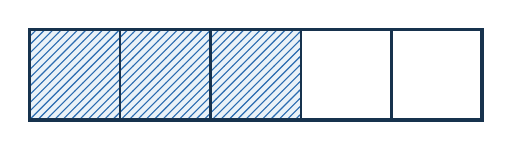
\begin{tikzpicture}[x=1.15cm, y=1.15cm]
  % Shaded parts: pale fill plus hatch pattern as a non-color cue
  \foreach \i in {0,1,2} {
    \fill[qraPale] (\i,0) rectangle (\i+1,1);
    \path[pattern=north east lines, pattern color=qraBlue] (\i,0) rectangle (\i+1,1);
  }
  % Internal part dividers and outer frame
  \foreach \i in {1,...,4} \draw[qra tick] (\i,0) -- (\i,1);
  \draw[qra axis] (0,0) rectangle (5,1);
\end{tikzpicture}
\end{document}
